\documentclass[11pt]{article}
\usepackage{tikz}
\usepackage{pifont}
\usepackage{amsmath}
\usepackage{marvosym}
\usepackage{verbatim}
\usepackage{listings}
\usepackage[utf8]{inputenc}
\usepackage{subfig}
\usepackage[switch,columnwise]{lineno}
\usepackage{amssymb}
\usepackage{enumitem}
\usepackage[nottoc,numbib]{tocbibind}
   
\usepackage{hyperref}
\hypersetup{
bookmarks=false,         % show bookmarks bar?
unicode=true,          % non-Latin characters in Acrobat's bookmarks
pdftoolbar=true,        % show Acrobat's toolbar?
pdfmenubar=true,        % show Acrobat's menu?
pdffitwindow=true,     % window fit to page when opened
pdfstartview={FitH},    % fits the width of the page to the window
pdftitle={Node allocators},    % title
pdfauthor={Marcelo Zimbres},     % author
pdfsubject={C++ allocators},   % subject of the document
pdfcreator={Marcelo Zimbres},   % creator of the document
pdfproducer={Marcelo Zimbres}, % producer of the document
pdfkeywords={allocators} {C++}, % list of keywords
pdfnewwindow=true,      % links in new window
colorlinks=true,        % false: boxed links; true: colored links
linkcolor=red,          % color of internal links
citecolor=red,        % color of links to bibliography
filecolor=red,      % color of file links
linktocpage=true,
urlcolor=blue           % color of external links
}

\lstset{
  language=C++,                 % the language of the code
  backgroundcolor=\color{white},   % choose the background color; you must add \usepackage{color} or \usepackage{xcolor}
  basicstyle=\footnotesize,        % the size of the fonts that are used for the code
  breakatwhitespace=false,         % sets if automatic breaks should only happen at whitespace
  breaklines=true,                 % sets automatic line breaking
  keywordstyle=\color{blue},       % keyword style
  captionpos=b,                    % sets the caption-position to bottom
  commentstyle=\color{blue},       % comment style
  deletekeywords={},            % if you want to delete keywords from the given language
  escapeinside={\%*}{*)},          % if you want to add LaTeX within your code
  extendedchars=true,              % lets you use non-ASCII characters; for 8-bits encodings only, does not work with UTF-8
  frame=no,                    % adds a frame around the code
  keepspaces=true,                 % keeps spaces in text, useful for keeping indentation of code (possibly needs columns=flexible)
  morekeywords={using},            % if you want to add more keywords to the set
  %numbers=left,                    % where to put the line-numbers; possible values are (none, left, right)
  numbersep=10pt,                   % how far the line-numbers are from the code
  numberstyle=\tiny\color{black}, % the style that is used for the line-numbers
  rulecolor=\color{black},         % if not set, the frame-color may be changed on line-breaks within not-black text (e.g. comments (green here))
  showspaces=false,                % show spaces everywhere adding particular underscores; it overrides 'showstringspaces'
  showstringspaces=false,          % underline spaces within strings only
  showtabs=false,                  % show tabs within strings adding particular underscores
  stepnumber=1,                    % the step between two line-numbers. If it's 1, each line will be numbered
  stringstyle=\color{red},     % string literal style
  tabsize=2,                       % sets default tabsize to 2 spaces
  title=\lstname                   % show the filename of files included with \lstinputlisting; also try caption instead of title
}

\colorlet{blah}{brown!60!black} % box color

\begin{document}

\date{}
\title{\bf Improving allocator interface for node-based containers}

\vspace{-2cm}
\maketitle
%\vspace{-2cm}

%\vspace{1cm}

\noindent
{\bf Document number}:  1 \\
{\bf Date}:  \today \\
{\bf Project}: Programming Language C++ \\
{\bf Author}: Marcelo Zimbres (\href{mailto:mzimbres@gmail.com}{mzimbres@gmail.com}) 

\vspace{1cm}

\noindent
{\bf Abstract: }This is a non-breaking proposal to the C++ standard that aims
to reduce allocator complexity, support realtime allocation and improve
performance of node-based containers by making a clear distinction between node
and array allocation in \texttt{std::allocator\_traits}.  Two new member
functions are proposed \texttt{allocate\_node} and \texttt{deallocate\_node}.
An example implementation is provided.

\tableofcontents

\vfill
%\newpage
%\twocolumn
%\linenumbers
\begin{flushright}
\noindent
{\it Size management adds undue difficulties \\
     and inefficiencies to any allocator design} \\
A. ALEXANDRESCU \\
\medskip
{\it }
\end{flushright}
\medskip

\section{Introduction}
\textsc{The importance} of linked data structures in computer science, like
trees and linked lists, cannot be over-emphasised, yet, in the last couple of
years it has become a common trend in C++ to move away from such data
structures due to their sub-optimal memory access patterns \cite{middleditch,
chandler, meyers}.  In fact, many people today prefer to use the flat
alternatives and pay $O(n)$ insertion time, than $O(1)$ at the cost of memory
fragmentation and unpredictable performance loss. Other domains, like {\it
realtime applications}, {\it embedded systems} or systems that aim {\it 24/7
availability}, cannot even afford the unpredictability introduced by memory
fragmentation and dynamic memory allocations in general.

To address these problems, we propose the complete split between array and
node allocations in the \texttt{std::allocator\_traits} by adding two new
functions, dedicated to node allocations, and a new typedef to inform when
node allocation should be used
\medskip
\begin{lstlisting}
template<class Alloc>
struct allocator_traits {
  using node_allocation_only = std::false_type
  pointer allocate_node(Alloc& a);
  void deallocate_node(Alloc& a, pointer);
};
\end{lstlisting}
The behaviour of these new members is better explained in section \ref{impact}.
These addition will allow the following configuration inside node-based
containers
\begin{itemize}
\item {\bf Array allocation only} \\
This is the status quo. When the allocator does not provide \texttt{allocate\_node},
the respective function in the \texttt{allocator\_traits} falls back to 
\texttt{allocate(1)}.
\item {\bf Node allocation only} \\
In this case the user is required the set the tpedef \texttt{node\_allocation\_only}
to \texttt{std::true\_type}. The user is not required to provide array allocation
in this case (i.e. \texttt{allocate(n)})
\item {\bf Array and node allocation together} \\
In this case the user provides \texttt{allocate\_node} but sets
\texttt{node\_allocation\_only} to \texttt{std::false\_type}.
\end{itemize}

These additions covers all use cases, is non-brekaing and very flexible.
For an alternative solution please see appendix \ref{alternative}.

\section{Motivation and scope}

\textsc{Some of} the motivations behind this proposal are
\begin{enumerate}

\item Support the most natural and one of the fastest allocation
scheme for linked data structures. In \texttt{libstd++} and
\texttt{libc++} for example, it is already possible (by chance) to use
this allocation technique, since $n$ is always $1$ on calls of
\texttt{allocate(n)}.

\item Node-based containers do not manage allocation sizes but
unnecessarily demand this feature from their allocators, with a cost
in performance and complexity. (Unordered associative containers use
sized allocations in addition to node allocation, which means they
need the sized version of \texttt{allocate} as well, but for purposes
other than node allocation).

\item Support hard-realtime allocation for node-based containers
through pre-allocation and pre-linking of nodes. This is highly
desirable to improve C++ usability in embedded systems.

\item State of the art allocators like \texttt{boost::node\_allocator}
\cite{boost} achieve great performance gains optimizing for the $n = 1$ case. 

\item Avoid wasted space behind allocations. It is pretty common that
allocators allocate more memory than requested to store information
like the size of the allocated block.

\item Keep nodes in as-compact-as-possible buffers, either on the
stack or on the heap, improving cache locality, performance and making
them specially useful for embedded programming.

\end{enumerate}

A question that naturally arises is: {\it Why not simply test
whether $n = 1$ and pass allocation to an appropriate
function internally?} For example

\medskip
\begin{lstlisting}
pointer allocate(size_type n)
{
  if (n == 1)
    return foo.allocate(); // Calls node allocation.
  return bar.allocate(n); // Calls regular allocate.
}
\end{lstlisting}

\noindent
The main reason why this is an undesirable approach is that the
possibility of having $n \ne 1$ means I have to handle allocations
with different sizes, which is exactly what I am trying to avoid for
reasons mentioned above i.e. reduce complexity, improve performance
etc. Additionally, test for the condition \texttt{if (n == 1)} is
pointless since it is always true on node allocation.

The simplification we are talking about comes from the fact that there
is no more need for an allocation algorithm or any fancy strategy
inside the allocator. We can simply build a singly linked list were
the nodes have the size demanded by the container, then allocation and
deallocation reduces to push and pop from the linked list.

\medskip
\begin{lstlisting}
pointer node_stack::pop()
{
  pointer q = avail; // The next free node
  if (avail)
    avail = avail->next;

  return q;
}

void node_stack::push(pointer p)
{
  p->next = avail;
  avail = p;
}

\end{lstlisting}

\medskip
\noindent
{\bf Further considerations}: The influence of fragmentation on
performance is well known on the C++ community and subject of many
talks in conferences therefore I am not going to repeat results here
for the sake of readability. The interested reader can refer to
\cite{chandler, meyers} for example.

For an allocator that explores the feature proposed here, please see
the project \cite{rtcpp}. For a general
talk on allocators and why size management is a problem
\cite{alexandrescu}. For related proposal, please see \cite{prop1}.

%\begin{figure}[ht]
%    \centering
%    \subfloat[]{ 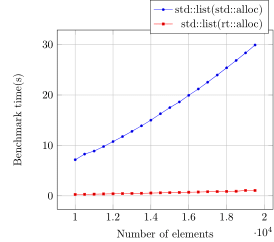
\includegraphics[scale=0.5]{fig/std_list_bench.png} }
%    \subfloat[]{ 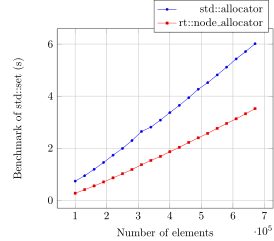
\includegraphics[scale=0.5]{fig/std_set_bench.png} }
%        \\
%    \caption[Benchmarks]
%    {Never slower than blah.}
%    \label{fig::bench}
%\end{figure}


\section{Impact on the Standard} \label{impact}

We require that all node based containers favor the overload
\texttt{allocate()} over \texttt{allocate(size\_type)}, for all node
allocations inside the container, whenever
\texttt{std::allocator\_traits} instructs them so, by means of a new
typedef
\medskip
\begin{lstlisting}
template<class Alloc>
struct allocator_traits {
  ...
  // Equal to Alloc::use_node_allocation if present
  // std::false_type otherwise.
  using node_allocation_only = std::false_type

  // Calls Alloc::allocate_node() if present otherwise
  // calls Alloc::allocate(n).
  pointer allocate_node(Alloc& a);

  // Calls Alloc::deallocate_node(pointer) if present
  // otherwise calls Alloc::deallocate(n).
  void deallocate_node(Alloc& a, pointer);
};
\end{lstlisting}
When \texttt{use\_node\_allocation} is not present in the allocator,
the typedef should default to \texttt{std::false\_type}.

The following containers are affected: \texttt{std::forward\_list},
\texttt{std::list}, \texttt{std::set}, \texttt{std::multiset},
\texttt{std::unordered\_set}, \texttt{std::unordered\_multiset},
\texttt{std::map}, \texttt{std::multimap},
\texttt{std::unordered\_map}, \texttt{std::unordered\_multimap}

\medskip
\noindent
{\bf Pure node-based}: As a result of this proposal all node based
containers mentioned above, with the exception of the unordered ones,
should support allocators that provide only the overload
\texttt{allocate()}.

\medskip
\noindent
{\bf Hybrid}: Unordered containers have to rebind twice, once
for node allocation and once for other internal data structures.
The rebound type used for node allocations should prefer the 
\texttt{allocate()} overload.

\section{Technical Specifications}

\section{Acknowledgment}

I would like thank people that give me any kind of feedback: Ville Voutilainen,
Nevin Liber, Daniel Gutson, Alisdair Meredith, David Krauss. Special thanks go
to Ion Gaztañaga, that suggested important changes in the original design.

\begin{thebibliography}{9}

  \bibitem{middleditch} Sean Middleditch, \url{http://www.open-std.org/jtc1/sc22/wg21/docs/papers/2015/p0038r0.html}
  \bibitem{chandler} Chandler Carruth, {\it Efficiency with Algorithms, Performance
  with Data Structures} (\url{https://www.youtube.com/watch?v=fHNmRkzxHWs})
  \bibitem{meyers} Scott Meyers, {\it Cpu Caches and Why You Care} (\url{https://www.youtube.com/watch?v=WDIkqP4JbkE})
  \bibitem{boost} \url{http://www.boost.org/doc/libs/1_58_0/boost/container/node_allocator.hpp}
  \bibitem{prop1} Ion Gazta\~ naga, \url{http://www.open-std.org/jtc1/sc22/wg21/docs/papers/2006/n2045.html}
  \bibitem{rtcpp} \url{https://github.com/mzimbres/rtcpp}
  \bibitem{alexandrescu} Andrei Alexandrescu, {\it std::allocator Is to Allocation what
  std::vector Is to Vexation} (\url{https://www.youtube.com/watch?v=LIb3L4vKZ7U})
  \bibitem{embedded} \url{http://www.open-std.org/pipermail/embedded/2014-December/000335.html}
  \bibitem{proplist} \url{https://groups.google.com/a/isocpp.org/forum/#!topic/std-proposals/ccwOpTxM_xE}

\end{thebibliography}

\appendix

\section{Alternative approach} \label{alternative}

\end{document}

